\documentclass[aspectratio=169,
hyperref={colorlinks,urlcolor=blue}
]{beamer}


%\usetheme{Pittsburgh}
\usetheme{default}
\usepackage{colortbl}%colored tables
%For using helvetica font:
\usepackage[scaled]{helvet}
\usepackage[T1]{fontenc}
\renewcommand\familydefault{\sfdefault}
\urlstyle{same} %sets the fonts for urls
\usepackage{pdfpages}
\usepackage{siunitx}
\usepackage{caption}
\usepackage{pifont}%for dings
\usepackage{pgfplots}%for 3d plotting
\pgfplotsset{compat = newest}
\usepackage{mathtools}%box in align env \Aboxed
\usepackage[american,smartlabels]{circuitikz}%for drawing circuits
\usepackage{multimedia}
\usepackage{animate}
\usepackage{xcolor}


\usetikzlibrary{arrows}
\usetikzlibrary {3d} 
\usetikzlibrary{decorations.markings, math}
\usetikzlibrary{intersections, pgfplots.fillbetween}
\usetikzlibrary {shapes.geometric} 


%\definecolor{myblue}{RGB}{5, 34, 150}
\definecolor{myblue2}{RGB}{5, 34, 150}
\definecolor{myblue}{RGB}{0,36,82}
\definecolor{myred}{RGB}{207, 2, 13}
\definecolor{mygreen}{RGB}{0, 158, 11}
\definecolor{myyellow}{RGB}{220,220,0}
\definecolor{qblue}{RGB}{0,36,82}
\definecolor{qgold}{RGB}{250,189,15}
\definecolor{qred}{RGB}{185,14,49}
\definecolor{cblue}{rgb}{0.13, 0.67, 0.8}
\definecolor{corange}{rgb}{0.8, 0.34, 0.0}
\definecolor{cpurple}{rgb}{0.54, 0.29, 0.42}

%%%%%%%%%%%% General settings
\setbeamercolor{frametitle}{fg=black}
\setbeamercolor{title}{fg=black}
\setbeamercolor{author}{fg=myblue2}

\beamertemplatenavigationsymbolsempty %no navigation controls at bottom of slides
%\setbeamertemplate{footline}[frame number]
\usefonttheme{professionalfonts} 
\setbeamerfont{title}{series=\bfseries,parent=structure}
\setbeamerfont{frametitle}{series=\bfseries,parent=structure}

%%%%%%%%%%%%Lists
\setbeamertemplate{itemize item}[circle] %{\color{myblue}$\circ$}
\setbeamertemplate{itemize subitem}{\color{myblue2}$\circ$}
\setbeamertemplate{itemize subsubitem}{\color{myblue2}$\cdot$}
\setbeamercolor{itemize item}{bg=myblue2,fg=myblue2}
\setbeamercolor{enumerate item}{bg=myblue2,fg=myblue2}
%%%%%%%%%%%%%%%%%%%%%%%%%%%%

%%%%%%%%%%%%Blocks
\setbeamertemplate{blocks}[rounded]
%Default block
\setbeamercolor{block title}{bg=myblue2, fg=white}
\setbeamercolor{block body}{bg=myblue2!10}
\setbeamerfont{block body}{size=\scriptsize}
\setbeamerfont{block title}{size=\scriptsize}
%Alert block
\setbeamercolor{block title alerted}{bg= myblue2, fg=white}
\setbeamercolor{block body alerted}{bg=myblue2!10}
\setbeamerfont{block body alerted}{size=\scriptsize}
\setbeamerfont{block title alerted}{size=\scriptsize}
%example block
\setbeamercolor{block title example}{bg=mygreen, fg=white}
\setbeamercolor{block body example}{bg=mygreen!10}
\setbeamerfont{block body example}{size=\scriptsize}
\setbeamerfont{block title example}{size=\scriptsize}
%%%%%%%%%%%%%%%%55


%%%%%%%%%%%%Figures and captions
\captionsetup{font=scriptsize,labelfont=scriptsize}
%\setbeamertemplate{caption}{\raggedright\insertcaption\par}
\newenvironment{capfig}[3]{\begin{figure}\includegraphics[width=#1\textwidth]{#2}\caption*{\textit{#3}}\end{figure}}{}

%\makeatother
%\setbeamertemplate{footline}
%{
%  \leavevmode%
%  \hbox{%
%  \begin{beamercolorbox}[wd=.4\paperwidth,ht=2.25ex,dp=1ex,center]{author in head/foot}%
%    \usebeamerfont{author in head/foot}\insertshortauthor
%  \end{beamercolorbox}%
%  \begin{beamercolorbox}[wd=.6\paperwidth,ht=2.25ex,dp=1ex,center]{title in head/foot}%
%    \usebeamerfont{title in head/foot}\insertshorttitle\hspace*{3em}
%    \insertframenumber{} / \inserttotalframenumber\hspace*{1ex}
%  \end{beamercolorbox}
%  }%
%  \vskip0pt%
%}
%\makeatletter

\makeatother
\setbeamertemplate{footline}
{
  \leavevmode%
  \hbox{%
\begin{beamercolorbox}[wd=.27\paperwidth,ht=2.25ex,dp=1ex,center]{author in head/foot}%
    \color{black}{\insertinstitute}
\end{beamercolorbox}
  \begin{beamercolorbox}[wd=.27\paperwidth,ht=2.25ex,dp=1ex,center]{author in head/foot}%
    \color{black}{\inserttitle}
  \end{beamercolorbox}%
  \begin{beamercolorbox}[wd=.27\paperwidth,ht=2.25ex,dp=1ex,center]{title in head/foot}%
    \color{black}{\insertshortauthor}
  \end{beamercolorbox}
  \begin{beamercolorbox}[wd=.27\paperwidth,ht=2.25ex,dp=1ex,center]{title in head/foot}%
    \hspace{.28\paperwidth}\color{black} \insertframenumber{} / \inserttotalframenumber\hspace*{1ex}
  \end{beamercolorbox}
  }%
  \vskip0pt%
}
\makeatletter

\setbeamertemplate{title page}
{
  \begin{tikzpicture}[remember picture,overlay]
    \def\barh{4}%15
  
    \draw[color=myblue2,line width=\barh] ([yshift=-0.5*\barh]current page.north west) -- ([yshift=-0.5*\barh,xshift=-0.67\paperwidth]current page.north east);
    \draw[color=myblue2,line width=\barh] ([yshift=-0.5*\barh,xshift=-0.67\paperwidth]current page.north east) -- ([yshift=-0.5*\barh,xshift=-0.34\paperwidth]current page.north east);
    \draw[color=myblue2,line width=\barh] ([yshift=-0.5*\barh,xshift=-0.34\paperwidth]current page.north east) -- ([yshift=-0.5*\barh]current page.north east); 
  
    \draw[color=myblue2,line width=\barh] ([yshift=0.5*\barh]current page.south west) -- ([yshift=0.5*\barh,xshift=-0.67\paperwidth]current page.south east);
    \draw[color=myblue2,line width=\barh] ([yshift=0.5*\barh,xshift=-0.67\paperwidth]current page.south east) -- ([yshift=0.5*\barh,xshift=-0.34\paperwidth]current page.south east);
    \draw[color=myblue2,line width=\barh] ([yshift=0.5*\barh,xshift=-0.34\paperwidth]current page.south east) -- ([yshift=0.5*\barh]current page.south east);
    %\node[left] at (current page.east) {
    %
\includegraphics[scale=0.1]{figures/coverpage}
    %};
  \end{tikzpicture}
  
  \usebeamerfont{title}\usebeamercolor[fg]{title}\inserttitle\par
  \usebeamerfont{subtitle}\usebeamercolor[fg]{subtitle}\insertsubtitle\par
  \vspace{2cm}
  \usebeamerfont{author}\usebeamercolor[fg]{author}\insertauthor\par
  \usebeamerfont{institute}\usebeamercolor[fg]{author}\insertinstitute\par
  \usebeamercolor[fg]{author}\par
  \usebeamercolor[fg]{titlegraphic}\inserttitlegraphic

} 

\setbeamertemplate{frametitle}{%
    \nointerlineskip%
        \par\hspace*{-\dimexpr0.5\paperwidth-0.5\textwidth}\textcolor{myblue2}{\rule{0.33\paperwidth}{6pt}}\textcolor{myblue2}{\rule{0.33\paperwidth}{6pt}}\textcolor{myblue2}{\rule{0.34\paperwidth}{6pt}} 
    \begin{beamercolorbox}[wd=\paperwidth,ht=0.75cm,dp=0.6ex]{frametitle}
        \hspace*{0.5cm}\strut\usebeamerfont{frametitle}\insertframetitle\strut
        %\hrule
    \end{beamercolorbox}%
    %%Line below:
%\par\hspace*{-\dimexpr0.5\paperwidth-0.5\textwidth}\textcolor{myblue}{\rule{\paperwidth}{0.4pt}}
     % <-- calculation of left margin width + rule
     %\textcolor{red}{\noindent\rule{\paperwidth}{2pt}}
}


%%%%%%%%%%%%Frame templates

%Slide with title
\newenvironment{titleframe}[1]
{\begin{frame}\frametitle{#1}\end{frame}}
{}

%Slide with title and itemize list:
\newenvironment{bulletframe}[1]
{\begin{frame}{#1} \itemize}
{\enditemize \end{frame}}

%Slide with two columns 50/50
\newenvironment{twocolframe}[3]
{\begin{frame}{#1}
 \begin{columns}[T]
 \column{0.5\textwidth}#2
 \column{0.5\textwidth}#3
 \end{columns}\end{frame}}{}

%Slide with two columns 60/40 <<<<<<<<<<<<<<<<<<<<<<  This one!
\newenvironment{twocolframesf}[3]
{\begin{frame}{#1}
 \begin{columns}[T]
 \column{0.6\textwidth}#2
 \column{0.4\textwidth}#3
 \end{columns}\end{frame}}{}
 
%Slide with two columns 70/30
\newenvironment{twocolframest}[3]
{\begin{frame}{#1}
 \begin{columns}[T] 
 \column{0.7\textwidth}#2
 \column{0.3\textwidth}#3
 \end{columns}\end{frame}}{} 
 
%Slide with two columns 40/60
\newenvironment{twocolframefs}[3]
{\begin{frame}{#1}
 \begin{columns}[T] 
 \column{0.4\textwidth}#2
 \column{0.6\textwidth}#3
 \end{columns}\end{frame}}{}
 
%Slide with two columns 70/30
\newenvironment{twocolframets}[3]
{\begin{frame}{#1}
 \begin{columns}[T] 
 \column{0.3\textwidth}#2
 \column{0.7\textwidth}#3
 \end{columns}\end{frame}}{} 

 
%Colloquium speaker (title, abstract, picture file, speaker name)
\newenvironment{colloquium}[5]
{
\begin{frame}{Colloquium: Friday 1:30pm in Stirling A}
\begin{columns}[T] 
 \column{0.8\textwidth}
 \textbf{#1}\\
 #2
 \column{0.2\textwidth}
 \capfig{#3}{#4}{#5}
 \end{columns}
\end{frame}
}
{} 

%%%%%%%%%%%%%Set Hyperref colors


\hypersetup{
  colorlinks=true,
  linkcolor=blue,    
  urlcolor=blue,     
  citecolor=blue      
}
%%%%%%%%%%%%%TOC bolding
\setbeamerfont{section in toc}{series=\bfseries}





%Frames:
% \twocolframesf 60/40 (fs, st, ts) 
% \titleframe
% bulletframe

%%%%%%%%%%%%%%%%%%%%%%%%%
%%%%%% START OF PRESENTATION %%%%%%
%%%%%%%%%%%%%%%%%%%%%%%%%

\title{Mathmatical Tools and Their Use In Physics}
\institute{Vectors and Calculus}
\author{Building Models to Describe our World}

\begin{document}

\begin{frame}
\titlepage
\thispagestyle{empty}
\end{frame}

%%%%%%%%%%%%%%%%%%%%%%%%%%%%%
\twocolframe{Outline}
{\tableofcontents[sections=1, subsectionstyle=show/show]}
{\tableofcontents[sections=2-3, subsectionstyle=show/show]}


%%%%%%%%%%%%

%%%%%%%%%%%%%%%%%%%%%%%%%%%
\section{Vectors}
\label{sec:vectors}
\title{Vectors}
\institute{Mathmatical Tools and Their Use In Physics}
\author{\insertsubsection}


%%%%%%%%%%%%%%%%%%%%%%%%%
%%%%%% Title slide %%%%%%
%%%%%%%%%%%%%%%%%%%%%%%%%
\begin{frame}
\titlepage
\thispagestyle{empty}
\end{frame}

%%%%%%%%%%%%%%%%%%%%%%%%%%%%%%%%
%%Advertisements and such %%%%%%
%%%%%%%%%%%%%%%%%%%%%%%%%%%%%%%%

%%%%%%%%%%%%%%
%\colloquium{title}
%{\small
%abstract
% }
%{scale}
%{figures/speaker}
%{\small \textbf{author},institute }
%

%%%%%%%%%%%%%%%%%%%%%%%%%%%%%%%%%%%%%%%%%%%%%%%%%%%%%%%%%%%%%%%%%%%%%%%%%%%%%%%%%%%%%%%
%%%%%%%%%%%%%%%%%%%%%%%%%%%%%%%%
%% Actual lecture slides  %%%%%%
%%%%%%%%%%%%%%%%%%%%%%%%%%%%%%%%



%%%%%%%%%%%%%%%%%%%%%%%%%%%%%%%%
\subsection{Coordinate systems}
\label{subsec:coordinatesystems}
\twocolframesf{Coordinate systems}
{
\begin{itemize}
\item Because we want to describe things in space, and we live in 3 dimensions!
\item In practice, we can often simplify and use 1D or 2D coordinate systems.
\item The most common type of coordinate system is a right-handed Cartesian coordinate system, where you must specify:
\begin{itemize}
\item 3 mutually perpendicular axes/directions (specify 2, the third is given by the right hand rule).
\item 1 fixed origin.
\end{itemize}
\item Using a coordinate system, can specify the position of a point using its \textbf{coordinates}.
\item Can you think of an example where you've used spherical coordinates?
\end{itemize}
}
{
\centering
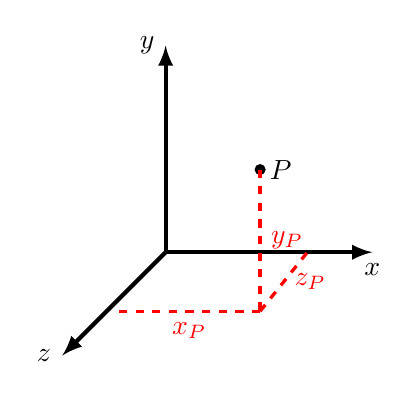
\begin{tikzpicture}[scale=1]
\tikzmath{
\R=1.5;
\f=0.5;
\fx=\f+1;
}
\scalebox{1.0}{

\coordinate (P) at (0.8*\R,0.7*\R);
\coordinate (PP) at (0.8*\R,-0.5*\R);
\coordinate (PX) at (0.8*\R*\fx,0);
\coordinate (PZ) at (-\f*0.8*\R,-0.5*\R);
 %axes:
 \draw[-latex, line width=1.5pt] (0,0) -- (1.75*\R,0) node[below]{$x$}; 
 \draw[-latex, line width=1.5pt] (0,0) -- (0,1.75*\R) node[left]{$y$}; 
 \draw[-latex, line width=1.5pt] (0,0) -- (-\f*1.75*\R,-\f*1.75*\R) node[left]{$z$};  
 
 %point
 \fill (P) circle(2pt);
 \node[right] at (P) {$P$};
 
 %dotted lines
 \draw[dashed,color=red,line width=1.2pt] (P) -- (PP) node[midway,right]{$y_P$};
 \draw[dashed,color=red,line width=1.2pt] (PP) -- (PX) node[midway,right]{$z_P$};
 \draw[dashed,color=red,line width=1.2pt] (PP) -- (PZ) node[midway,below]{$x_P$};
}
\end{tikzpicture}
\captionof*{figure}{\textit{A \textbf{right-handed} Cartesian coordinate system, where $\hat x \times \hat y = \hat z$. ($\hat z$ is out of the page). The point $P$ has coordinates $(x_P,y_P,z_P)$.}}
}

%%%%%%%%%%%%%%%%%%%%%%%%%%%%%%%%
\subsection{Vector basics}
\label{subsec:vectorbasics}
\twocolframest{Vectors}
{
\begin{itemize}
\item Vectors are arrows with a magnitude and a direction.
\item They are useful for describing quantities with a magnitude and a direction:
\begin{itemize}
\item A displacement.
\item A velocity.
\item A force.
\item An angular velocity.
\end{itemize}
\item We can describe a vector by specifying its \textbf{components}, or its magnitude and direction(s) (in 3D, need magnitude and two angles).
\item Notation:
\end{itemize}
\begin{align*}
\vec v = v_x\hat x+v_y\hat y+v_z\hat z=(v_x,v_y,v_z)=\begin{pmatrix}
v_x\\v_y\\v_z
\end{pmatrix}
\end{align*}
}
{
\centering
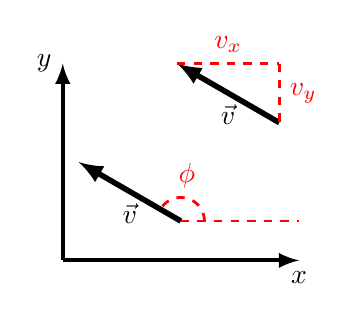
\begin{tikzpicture}[scale=1]
\tikzmath{
\L=2.5;
\v=1.5;
}
\scalebox{1.0}{

 \coordinate (P1) at (1.1*\L,0.7*\L);
 \coordinate (P2) at ($(P1)+(-0.5*\L,-0.5*\L)$);
 
 %axes:
 \draw[-latex, line width=1.5pt] (0,0) -- (1.2*\L,0) node[below]{$x$}; 
 \draw[-latex, line width=1.5pt] (0,0) -- (0,\L) node[left]{$y$}; 
 
 \draw[-latex,line width=2pt] (P1) -- ($(P1)+(150:\v)$) node[midway,below]{$\vec v$};
 \draw[dashed,line width=1pt,color=red] ($(P1)+(150:\v)$) -- ($(P1)+(150:\v)+cos(30)*(\v,0)$) node[midway, above] {$v_x$};
 \draw[dashed,line width=1pt,color=red] ($(P1)+(150:\v)+cos(30)*(\v,0)$) --(P1) node[midway, right] {$v_y$};
 
 \draw[-latex,line width=2pt] (P2) -- ($(P2)+(150:\v)$) node[midway,below]{$\vec v$};
 \draw[dashed,line width=1pt,color=red] (P2) -- ($(P2)+(0:\v)$);
 \draw[dashed,line width=1pt,color=red] ($(P2)+(0.2*\v,0)$) arc (0:150:0.2*\v) node[midway, above] {$\phi$};;
}
\end{tikzpicture}
\captionof*{figure}{\textit{A vector in 2D can be specified by two Cartesian components ($v_x,v_y$) or its length, $v$, and an angle with respect to the $x$ direction, $\phi$.}}
}


%%%%%%%%%%%%%%%%%%%%%%%%%%%%%%%%




%%%%%%%%%%%%%%%%%%%%%%%%%%%%%%%%
\begin{bulletframe}{Algebra with vectors}
 \item You can multiply/divide a vector by \textbf{a scalar}.
 \item You cannot add a scalar to a vector (as with anything, you cannot add oranges and apples).
 \item You can add/subtract two vectors (of the same dimensions, e.g. 2D or 3D).
 \item Two ways to multiply vectors:
 \begin{itemize}
   \item Scalar/dot product $\rightarrow$ the result is a scalar.
 \item Vector/cross product $\rightarrow$ the results is a vector (and this requires 3D and a flexible wrist).
 \end{itemize}
\end{bulletframe}

%%%%%%%%%%%%%%%%%%%%%%%%%%%%%%%%
%%%%%%%%%%%%%%%%%%%%%%%

%%%%%%%%%%%%%%%%%%%%%%%%%%%%%%%%
\twocolframesf{Vector addition and vector equations}
{
\scriptsize
\begin{itemize}
\item To add vectors $\vec a$ and $\vec b$:
\begin{itemize}
\scriptsize
\item Graphically, place them head to tail.
\item Algebraically, add the components together.
\end{itemize}
\item The ``unit vector'' notation for a vector is just vector addition:
\begin{align*}
\vec a = a_x \hat x + a_y \hat y
\end{align*}
\item<2-> \textbf{An equation with vectors is a short-hand for equations between components:}
\begin{align*}
\vec c = \vec a + 2\vec b
\end{align*}
\emph{is the same as the two independent equations:}
\begin{align*}
c_x &= a_x + 2b_x\\
c_y &= a_y+2b_y
\end{align*}
\end{itemize}
}
{
\centering
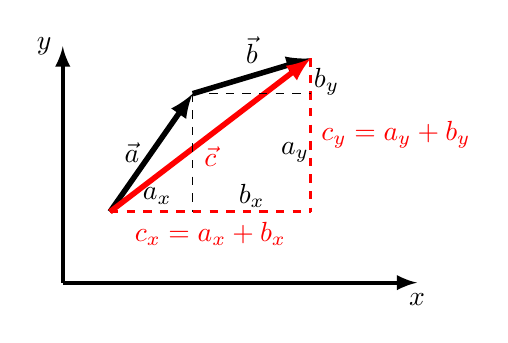
\begin{tikzpicture}[scale=1]
\tikzmath{
\L=3.;
\u=\L/2;
}
\scalebox{1.0}{

 \coordinate (P) at (0.2*\L,0.3*\L);
 \coordinate (PA) at ($(P)+(0.7*\u,\u)$);
 \coordinate (PC) at ($(PA)+(1.0*\u,0.3*\u)$);
 \coordinate (PAX) at ($(P)+(0.7*\u,0)$);
 \coordinate (PBY) at ($(PC)+(0,-0.3*\u)$);
 %axes:
 \draw[-latex, line width=1.5pt] (0,0) -- (1.5*\L,0) node[below]{$x$}; 
 \draw[-latex, line width=1.5pt] (0,0) -- (0,\L) node[left]{$y$}; 
 
 \draw[-latex,line width=2pt] (P) -- (PA) node[midway,left]{$\vec a$};
 \draw[-latex,line width=2pt] (PA) -- (PC) node[midway,above]{$\vec b$};
 \draw[-latex,line width=2pt, color=red] (P) -- (PC) node[midway,below]{$\vec c$};
 
 \only<2>{
 \draw[dashed, line width=1.0, color=red] (P) -- ($(P)+(1.7*\u,0)$) node[midway,below]{$c_x=a_x+b_x$};
 \draw[dashed, line width=1.0, color=red] (PC) -- ($(PC)+(0,-1.3*\u)$)node[midway,right]{$c_y=a_y+b_y$};
 
 \draw[dashed] (PA) -- (PAX);
 \draw[dashed] (PA) -- (PBY);
 
 \node at ($(PAX)+(-0.3*\u,0.2)$) {$a_x$};
 \node at ($(PAX)+(0.5*\u,0.2)$) {$b_x$};
 \node at ($(PBY)+(-0.2,-0.5*\u)$) {$a_y$};
 \node at ($(PBY)+(0.2,0.1*\u)$) {$b_y$};
 }
}
\end{tikzpicture}
\captionof*{figure}{\textit{A graphical illustration of $\vec c = \vec a + \vec b$.}}
}

%%%%%%%%%%%%%%%%%%%%%%%%%%%%%%%%
\subsection{Scalar Product}
\label{subsec:scalarproduct}
\twocolframest{Scalar product}
{
%\scriptsize
\begin{itemize}
\item Scalar product is a sum of the components of the two vectors multiplied together (commutative):
\begin{align*}
\vec a \cdot \vec b = a_xb_x+a_yb_y+a_zc_z=\vec b \cdot \vec a
\end{align*}
\item It is also proportional to the cosine of the angle between the vectors (if these are placed tail to tail):
\begin{align*}
\vec a \cdot \vec b = ab\cos\theta
\end{align*}
\item It is thus zero if two vectors are perpendicular to each other, $\cos(90)=0$
\item By knowing the components of two vectors, you can determine their scalar product, and then the angle between the two vectors
\end{itemize}
}
{
\centering
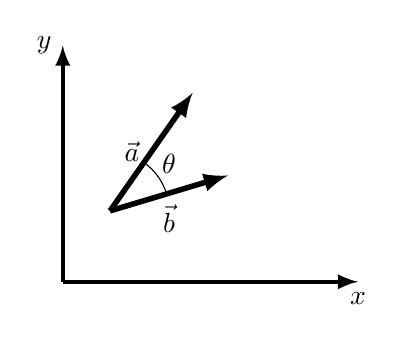
\begin{tikzpicture}[scale=1]
\tikzmath{
\L=3.;
\u=\L/2;
}
\scalebox{1.0}{

 \coordinate (P) at (0.2*\L,0.3*\L);
 \coordinate (PA) at ($(P)+(0.7*\u,\u)$);
 \coordinate (PB) at ($(P)+(1.0*\u,0.3*\u)$);

 %axes:
 \draw[-latex, line width=1.5pt] (0,0) -- (1.25*\L,0) node[below]{$x$}; 
 \draw[-latex, line width=1.5pt] (0,0) -- (0,\L) node[left]{$y$}; 
 
 \draw[-latex,line width=2pt] (P) -- (PA) node[midway,left]{$\vec a$};
 \draw[-latex,line width=2pt] (P) -- (PB) node[midway,below]{$\vec b$};
 
 \node at ($(P)+(0.5*\u,0.4*\u)$){$\theta$};
 \path[clip] (P) -- (PA) -- (PB) -- cycle;
 \draw ($(P)+(0.5*\u,0)$) arc (0:90:0.5*\u);

 

}
\end{tikzpicture}
\captionof*{figure}{\textit{The scalar product between vectors depends on the angle between them when they are placed tail to tail.}}
}

%%%%%%%%%%%%%%%%%%%%%%%%%%%%%%%%

%%%%%%%%%%%%%%%%%%%%%%%%%%%%%%%%
\subsection{Cross-Product}
\label{subsec:crossproduct}
\twocolframesf{Cross-product}
{
\scriptsize
\begin{itemize}
\item The cross product gives a \textbf{vector} that is perpendicular to the original two vectors (not commutative):
\begin{align*}
\vec a \times \vec b = \vec c = -\vec b \times \vec a
\end{align*}
\item The magnitude is related to the sine of the angle between the two original vectors:
\begin{align*}
||\vec a \times \vec b ||= ab\sin\theta
\end{align*}
\item The cross-product is zero if the two vectors are parallel or anti-parallel ($\sin 0 =0$)
\item The direction of the cross product can be found using the right hand rule
\item Cross products are always in 3D
\end{itemize}
}
{
\scriptsize
You can find the components of the cross product algebraically:
\begin{align*}
\vec a \times \vec b =\begin{pmatrix}
           a_yb_z - a_z b_y\\
           a_zb_x - a_x b_z\\
           a_xb_y - a_y b_x\\
         \end{pmatrix}
\end{align*}
or using the right-hand rule for cross-products for the direction:
\capfig{1}{../figures/Math/righthandrule}{}
}
\label{fig:math:righthandrule}
%%%%%%%%%%%%%%%%%%%%%%%%%%%%%%%%


%%%%%%%%%%%%%%%%%%%%%%%%%%%%%%%%
\twocolframesf{Scalar and cross product in action}
{

Scalar product:
\begin{itemize}
\item Maximal when two vectors are parallel.
\item Zero when two vectors are perpendicular.
\item Application: ``Work''.
\end{itemize}
\vspace{1cm}
Cross product:
\begin{itemize}
\item Maximal when two vectors are perpendicular.
\item Zero when two vectors are parallel.
\item Application: ``Torque''.
\end{itemize}
}
{
\centering
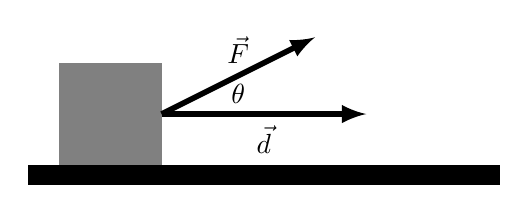
\begin{tikzpicture}[scale=1]
\tikzmath{
\L=3.;
\w=0.25;
\a=1.3;
}
\scalebox{1.0}{

\fill (-\L,-\w) rectangle (\L,0);
\fill[black!50] (-2*\a,0) rectangle (-\a,\a);

\draw[-latex,line width=2pt] (-\a,\a/2) -- +(1.5*\a,0.75*\a) node[midway,above] {$\vec F$};
\draw[-latex,line width=2pt] (-\a,\a/2) -- +(2*\a,0) node[midway,below] {$\vec d$};
\node at ($(-\a,\a/2)+(0.75*\a,0.2*\a)$) {$\theta$};
}
\end{tikzpicture}
\captionof*{figure}{\textit{The scalar product between force and displacement, $W=\vec F \cdot \vec d=Fd\cos\theta$ (Work) tells us about the change in speed.}}

\centering
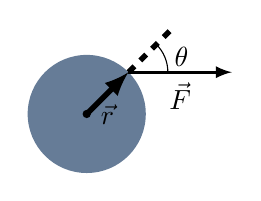
\begin{tikzpicture}[scale=1]
\tikzmath{
\R=0.75;
}
\scalebox{1.0}{

\fill[color=myblue!60] circle (\R);
\fill[] circle (1.5pt);

\draw[-latex, line width = 2pt] (0,0) -- (45:\R) node[midway, below]{$\vec r$};
\draw[dashed, line width = 2pt] (45:\R) -- + (45:\R);
\draw ($(45:\R)+(0.5,0)$) arc (0:45:0.5) node[midway, right]{$\theta$};
\draw[-latex, line width = 1pt] (45:\R) -- + (1.75*\R,0) node[midway, below]{$\vec F$};

}
\end{tikzpicture}
\captionof*{figure}{\textit{The magnitude of cross product between a force, $\vec F$, and the position vector, $\vec r$, where the force is applied tells us the angular acceleration of an object: $||\vec r \times \vec F||=rF\sin\theta$.}}

}


%%%%%%%%%%%%%%%%%%%%%%%%%%%%%%%%
\subsection{Vectors to indicate rotation}
\label{subsec:rotationvectors}
\twocolframesf{Vectors to indicate rotation}
{
\begin{itemize}
\item Suppose that you need to describe a rotating wheel to someone over the phone.
\item You need to specify:
\begin{itemize}
\item The axis of rotation (a line)
\item How fast (e.g. rotations per minute)
\item Which direction (clockwise/counter clockwise) about that axis
\end{itemize}
\item This can be specified by an “axial vector”, and the “right hand rule for axial vectors”:
\begin{itemize}
\item The vector is co-linear with the axis of rotation
\item The magnitude is proportional to rotational speed
\item The direction of the vector is given by the right hand rule for axial vectors.
\end{itemize}
\end{itemize}
}
{
\capfig{0.75}{../figures/Math/righthandruleaxial}{}
\label{fig:math:righthandruleaxial}
\capfig{0.9}{../figures/Math/carwheelrotation}{}
\label{fig:math:carwheelrotation}
}
%%%%%%%%%%%%%%%%%%%%%%%%%%
\section{Derivatives}
\label{sec:derivatives}
\title{Derivatives}
\institute{Mathmatical Tools and Their Use In Physics}
\author{\insertsubsection}
%%%%%%%%%%%%%%%%%%%%%%%%%%%%%%%%%%%


\begin{frame}
\titlepage
\thispagestyle{empty}
\end{frame}

%%%%%%%%%%%%%%%%%%%%%%%%%%%%%%%%%%%
\subsection{Functions}
\label{subsec:functions}
\begin{bulletframe}{Functions}
 \item We will mostly concern ourselves with functions that are mappings from a set of independent variables (x, y , z, t) to (usually) a real number.
 \item Examples of functions in physics:
 \begin{itemize}
  \item Position as a function of time for an accelerating object: $x(t)=x_0+v_{x0}t+\frac{1}{2}a_xt^2$
 \item The restoring force from a spring: $F(x) = -kx$
 \item The potential energy from gravity near Earth’s surface: $V(h) = mgh$ 
 \item The electric field from a point charge at the origin: 
 \begin{align*}
 \vec E(x,y,z) =\frac{kq}{x ^2+y^2+z^2}\hat r \quad \text{(this is one is not a mapping to a real number!)}
 \end{align*} 
\item etc….
 \end{itemize}
\end{bulletframe}


%%%%%%%%%%%%%%%%%%%%%%%%%%%%%%%%
\begin{bulletframe}{Properties of a function}
 \item When you encounter a function, ask yourself:
 \begin{itemize}
  \item Is the function ever equal to zero (what are its “roots”)?
 \item Is the function continuous for all values of the independent variables?
 \item Are there maxima/minima in the function?
 \item Is the function always defined? This is especially important in physics. We need functions to represent physical quantities, so we need to understand when they are undefined
 \end{itemize}
 \item The best thing to do is to sketch out the function to get a sense of it $\rightarrow$ There are many online tools (e.g. Wolfram alpha, Jupyter notebooks, etc)
\end{bulletframe}


%%%%%%%%%%%%%%%%%%%%%%%%%%%%%%%%



%%%%%%%%%%%%%%%%%%%%%%%%%%%%%%%%
\subsection{The Derrivative}
\label{subsec:thederrivative}
\twocolframesf{The derivative}
{
\begin{itemize}
\item The derivative of a function, $f(x)$, is the slope of the function (``rise over run'').
\item It tells us how steep the function is, namely, how fast it is increasing or decreasing, or neither $\rightarrow$ the rate of change of $f(x)$ with respect to $x$.
\item The derivative of a function is a function.
\item Different notations for the derivative of $f(x)$ with respect to $x$: \\\
$f'(x)$, $\frac{df}{dx}$, $\frac{d}{dx} f(x)$   
\item It tells us the (tangent of the) angle which the tangent to the function makes with the x-axis.
\end{itemize}
}
{
\centering
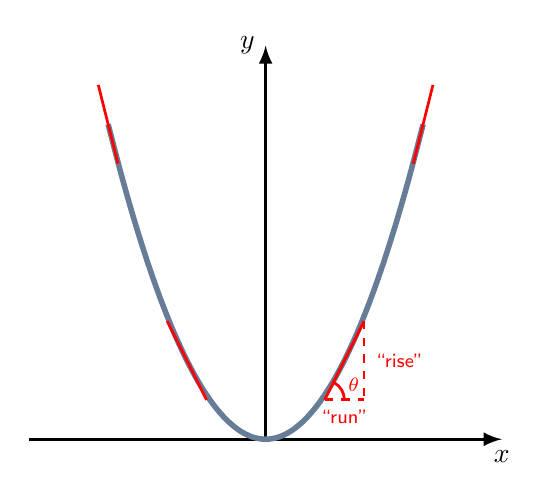
\begin{tikzpicture}[scale=1]
\tikzmath{
}
\scalebox{1.0}{
 \coordinate (P) at (1,1);
 \coordinate (P2) at (-1,1);
 \coordinate (P3) at (-2,4);
 \coordinate (P4) at (2,4);
 %axes:
 \draw[-latex, line width=1.25pt] (-3,0) -- (3,0) node[below]{$x$}; 
 \draw[-latex, line width=1.25pt] (0,0) -- (0,5) node[left]{$y$}; 
 
 %function
 \draw[scale=1, domain=-2.:2., smooth, variable=\x, line width=2,color=myblue!60] plot ({\x}, {\x*\x});
 
 
 \draw[red, line width=1] ($(P)-(0.25,0.5)$) -- ($(P)+(0.25,0.5)$);
 \draw[red, dashed, line width=1] ($(P)-(0.25,0.5)$) --  +(0.5,0) node[midway,below]{\scriptsize ``run''};
 \draw[red, dashed, line width=1] ($(P)+(0.25,0.5)$) --  +(0,-1) node[midway,right]{\scriptsize ``rise''};
 
 \draw[red, line width =1] ($(P)-(0.25,0.5)+(0.25,0)$) arc (0:60:0.25) node[midway,above=2pt,right=-1.5pt] {\scriptsize $\theta$};
 
 \draw[red, line width=1] ($(P2)-(0.25,-0.5)$) -- ($(P2)+(0.25,-0.5)$);
 \draw[red, line width=1] ($(P3)-(0.125,-0.5)$) -- ($(P3)+(0.125,-0.5)$);
 \draw[red, line width=1] ($(P4)-(0.125,0.5)$) -- ($(P4)+(0.125,0.5)$);
}
\end{tikzpicture}
\captionof*{figure}{\textit{The derivative of the function is given by the ``rise over the run''. This corresponds to the tangent of the angle that the tangent to the function makes at that point.}}
}

%%%%%%%%%%%%%%%%%%%%%%%%%%%%%%%%
\twocolframesf{The derivative is the \emph{instantaneous} rate of change of a function}
{
\begin{itemize}
\item It tells us how much $f(x)$ changes, when we change $x$, at some point $x$.
\item That is, it tells us the value of $\Delta f$ if we go from $x$ to $x+\Delta x$.
\item Suppose that we choose two points, $x_1$  and $x_2$, separated by a distance $\Delta x$:
\begin{align*}
\Delta x &= x_2-x_1,\quad f(x_1) = f_1, \quad f(x_2)=f_2\\
\Delta f &=f_2-f_1\\
\therefore f'(x) &= \frac{df}{dx}=\lim_{\Delta x\to 0}\frac{\Delta f}{\Delta x}=\lim_{\Delta x\to 0}\frac{f(x+\Delta x)-f(x)}{\Delta x}
\end{align*}
 
\end{itemize}
}
{
\centering
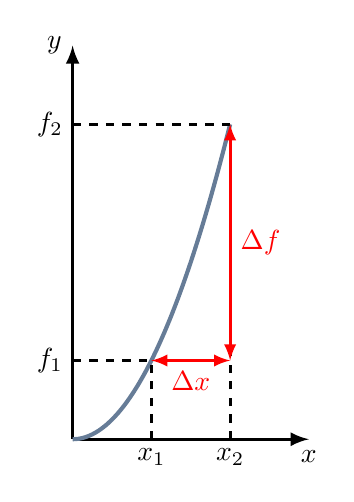
\begin{tikzpicture}[scale=1]
\tikzmath{
}
\scalebox{1.0}{
 \coordinate (P) at (1,1);

 %axes:
 \draw[-latex, line width=1.25pt] (0,0) -- (3,0) node[below]{$x$}; 
 \draw[-latex, line width=1.25pt] (0,0) -- (0,5) node[left]{$y$}; 
 
 %function
 \draw[scale=1, domain=0.:2., smooth, variable=\x, line width=1.5,color=myblue!60] plot ({\x}, {\x*\x});
 
 \node[below] at (1,0) {$x_1$};
 \node[below] at (2,0) {$x_2$};
 \node[left] at (0,1) {$f_1$};
 \node[left] at (0,4) {$f_2$};
 
 \draw[dashed,line width =1] (1,0) -- (1,1);
 \draw[dashed,line width =1] (2,0) -- (2,4);
 \draw[dashed,line width =1] (0,1) -- (1,1);
 \draw[dashed,line width =1] (0,4) -- (2,4);
 
 \draw[latex-latex,red, line width=1] (1,1) -- +(1,0) node[midway,below]{$\Delta x$};
 \draw[latex-latex,red, line width=1] (2,4) -- +(0,-3) node[midway,right]{$\Delta f$};
}
\end{tikzpicture}
\captionof*{figure}{\textit{The derivative of the function is given by $\frac{\Delta f}{\Delta x}$ in the limit where $\Delta x \to 0$.}}
}

%%%%%%%%%%%%%%%%%%%%%%%%%%%%%%%%



%%%%%%%%%%%%%%%%%%%%%%%%%%%%%%%%
\subsection{How to find a derivative}
\label{subsec:howtofindder}
\begin{frame}{How to find a derivative}
\begin{itemize}
\item You’ll learn in calculus (the textbook shows how to do derive it for the case of $f(x)=x^2$).
\item For now, you need to know where to look them up, and how to apply the rules:
\end{itemize}
\centering
\only<1>{
\begin{tabular}{l l}
\textbf{Function, $f(x)$} & \textbf{Derivative, $f'(x)$}\\
\hline\hline
$f(x)=a$ & $f'(x)=0$ \\
$f(x)=x^n$ & $f'(x)=nx^{n-1}$ \\
$f(x)=\sin(x)$ & $f'(x)=\cos(x)$ \\
$f(x)=\cos(x)$ & $f'(x)=-\sin(x)$ \\
$f(x)=\tan(x)$ & $f'(x)=\frac{1}{\cos^2(x)}$ \\
$f(x)=e^x$ & $f'(x)=e^x$ \\
$f(x)=\ln(x)$ & $f'(x)=\frac{1}{x}$ \\
\hline
\end{tabular}
\captionof*{table}{\label{tab:Calculus:commonders}Common derivatives of functions.}}
\only<2>{
\begin{tabular}{l l}
\textbf{Function, $h(x)$} & \textbf{Derivative, $h'(x)$}\\
\hline\hline
$h(x)=f(x)+g(x)$ & $h'(x)=f'(x)+g'(x)$ \\
$h(x)=f(x)-g(x)$ & $h'(x)=f'(x)-g'(x)$ \\
$h(x)=f(x)g(x)$ & $h'(x)=f'(x)g(x)+f(x)g'(x)$ (The product rule) \\
$h(x)=\frac{f(x)}{g(x)}$ & $h'(x)=\frac{f'(x)g(x)-f(x)g'(x)}{g^2(x)}$ (The quotient rule)\\
$h(x)=f(g(x))$ & $h'(x)=f'(g(x))g'(x)$ (The Chain Rule) \\
\hline
\end{tabular}
\captionof*{table}{\label{tab:Calculus:combders}Derivatives of combined functions.}
}
\end{frame}

%%%%%%%%%%%%%%%%%%%%%%%%%%%%%%%%



%%%%%%%%%%%%%%%%%%%%%%%%%%%%%%%%
\begin{bulletframe}{Inifinitesimals - Calculus notation}
\scriptsize
\item Calculus usually involves asking what happens when something is very small
\item The derivative is:
\begin{align*}
f'(x) =\lim_{\Delta x\to 0}\frac{\Delta f}{\Delta x}
\end{align*}
\item We write this as:
\begin{align*}
f'(x) =\frac{df}{dx}
\end{align*}
\item You can really think of $dx$ as a very small $\Delta x$, and $df$ as the \emph{correspondingly} small $\Delta f$.
\item You can multiply them out:
\begin{align*}
f'(x) dx=df
\end{align*}
\item You can cancel them out:
\begin{align*}
\frac{df}{dg}\frac{dg}{dx}=\frac{df}{dx}
\end{align*}
\item This works because 
\begin{align*}
dx=\lim_{\Delta x\to 0} \Delta x
\end{align*}
(your math friends are cringing…) 
\end{bulletframe}


%%%%%%%%%%%%%%%%%%%%%%%%%%%%%%%%
\subsection{Functions of multiple variables}
\label{subsec:multvarfuncs}
\twocolframe{Functions of multiple variables}
{
\only<1>{
\begin{itemize}
\item Many quantities depend on where you are in space (i.e. a function of x,y,z).
\item These become difficult to visualize...
\item We have to define the rate of change of the function in any direction...
\item In the plot, at point $P$:
\begin{itemize}
\item The function decreases as $x$ increases (if $y$ is held fixed, dashed red line).
\item The function increases as $y$ increases (if $x$ is held fixed, solid red line).
\end{itemize}
\end{itemize}
}
\only<2>{
\begin{itemize}
\item The partial derivative of $f(x, y)$ with respect to $x$ tells us the rate of change of $f$ as a function of $x$ if we hold $y$ constant (following the dashed line).
\item The partial derivative of $f(x, y)$ with respect to $y$ tells us the rate of change of $f$ as a function of $y$ if we hold $x$ constant (following the solid line).
\item There are $n$ partial derivatives if there are $n$ independent variables.
\item Each partial derivative is a new function of the $n$ variables.
\end{itemize}
}
\only<3>{
Notation:
\begin{align*}
f(x,y)&=x^2-2y^2\\
\therefore\frac{\partial f}{\partial x}&=\frac{\partial}{\partial x}x^2-2y^2=2x\\
\therefore\frac{\partial f}{\partial y}&=\frac{\partial}{\partial y}x^2-2y^2=-4y;
\end{align*}
\begin{itemize}
\item Pronounced ``die f by die x''.
\item Calculate a partial derivative exactly the same way that you would a normal derivative (treat all other independent variables as constants).
\end{itemize}
}

}
{
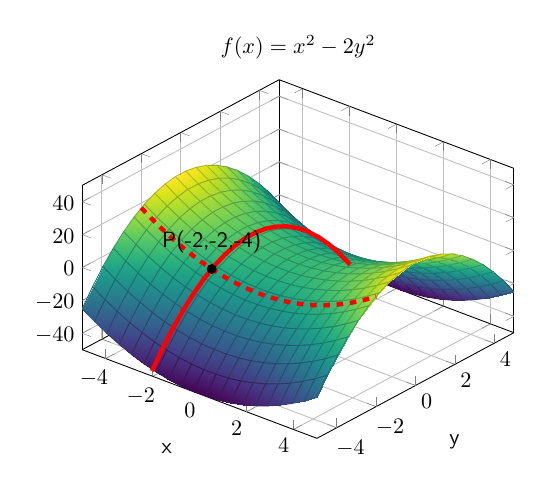
\begin{tikzpicture}[scale=0.8]

\begin{axis}[
  colormap/viridis,  
  view = {40}{40},
	xmax = 5,
	xmin = -5,
	ymax = 5, 
	ymin = -5, 
	zmax = 50, 
	zmin = -50,
	xtick = {-4,-2,0,2,4},
	ytick = {-4,-2,0,2,4},
	ztick = {-40,-20,0,20,40},
	xlabel={x},
	ylabel={y},
	title={$f(x)=x^2-2y^2$},
	grid]
	

\addplot3 [
	domain=-5:5,
	domain y = -5:5,
	samples = 20,
	samples y = 20,
	surf,
	shader =faceted interp] {x^2 -2*y^2};
	
\addplot3 [
	domain=-5:5,
	samples = 20,
	samples y = 1,
	line width =2,
	color=red,
	dashed,
	smooth] (x,-2,{x^2 -8});
	
\addplot3 [
	domain y =-5:5,
	samples = 1,
	samples y = 20,
	line width =2,
	color=red,
	smooth] (-2,y,{4 -2*y^2});	
	
\node[label={P(-2,-2,-4)}] at (-2,-2,-4) {};
\draw plot [mark=*, mark size=2] coordinates{(-2,-2,-4)}; 

\end{axis}

\end{tikzpicture}
\captionof*{figure}{\textit{A point, $P$, is on the surface given by $f(x,y)=x^2-2y^2$.}}
}


%%%%%%%%%%%%%%%%%%%%%%%%%%%%%%%%
\subsection{The gradient vector}
\label{subsec:gradientvector}
\twocolframe{The gradient vector}
{
\begin{itemize}
\item From the partial derivatives, we know how the function changes along the x and y directions.
\item The gradient tells us the direction in which the function changes the fastest, with components given by the partial derivatives.
\item It is a vector whose magnitude tells us how fast the function is changing in the direction of maximal change.
\begin{align*}
\nabla f(x,y) &= \frac{\partial f}{\partial x} \hat x + \frac{\partial f}{\partial y}\hat y\\
&=2x\hat x - 4y \hat y = (-4,8)
\end{align*}
\end{itemize}
}
{
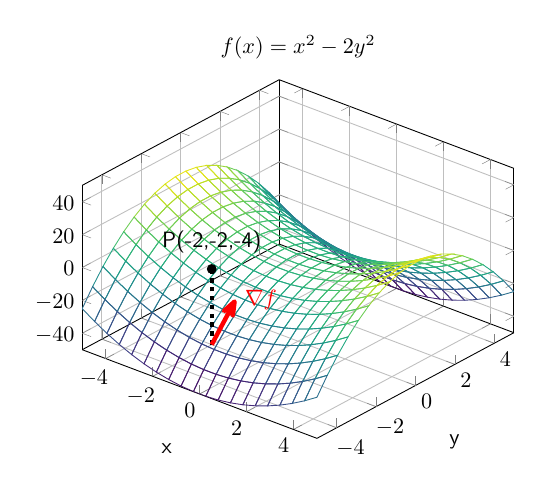
\begin{tikzpicture}[scale=0.8]
\usetikzlibrary {arrows.meta} 
\begin{axis}[
  colormap/viridis,  
  view = {40}{40},
	xmax = 5,
	xmin = -5,
	ymax = 5, 
	ymin = -5, 
	zmax = 50, 
	zmin = -50,
	xtick = {-4,-2,0,2,4},
	ytick = {-4,-2,0,2,4},
	ztick = {-40,-20,0,20,40},
	xlabel={x},
	ylabel={y},
	title={$f(x)=x^2-2y^2$},
	grid]
	

\addplot3 [
	domain=-5:5,
	domain y = -5:5,
	samples = 20,
	samples y = 20,
	mesh,
	%fill opacity=0.5,
	shader =faceted interp] {x^2 -2*y^2};
	
\draw[line width=2pt,dotted] (-2,-2,-50) -- (-2,-2,-4)	;
\node[label={P(-2,-2,-4)}] at (-2,-2,-4) {};
\draw plot [mark=*, mark size=2] coordinates{(-2,-2,-4)}; 
\draw[line width=2pt,red,-{Stealth[round]}] (-2,-2,-50)--(-3.5,1,-50) node[right]{$\nabla f$};

\end{axis}

\end{tikzpicture}
\captionof*{figure}{\textit{A vector parallel to the gradient vector is projected in the $xy$-plane. It points in the direction of most rapid increase.}}
}
%%%%%%%%%%%%%%%%%%%%%%%%%%%%%%%%



%%%%%%%%%%%%%%%%%%%%%%%%%%
\section{Integrals}
\label{sec:integrals}
\title{Integrals}
\institute{Mathmatical Tools and Their Use In Physics}
\author{\insertsubsection}
%%%%%%%%%%%%%%%%%%%%%%%%%%%%%%%%%%%


\begin{frame}
\titlepage
\thispagestyle{empty}
\end{frame}

%%%%%%%%%%%%%%%%%%%%%%%%%%%%%%%%%%%
\subsection{Rod examples}
\label{subsec:rodexamples}
\twocolframest{Example: The mass of a uniform rod}
{
\begin{itemize}
\scriptsize
\item Suppose that the rod has length L and mass M
\item We can define a linear mass density, $\mu$, (mass per unit length):
\begin{align*}
\mu=\frac{M}{L}
\end{align*}
\item A small section of rod, with length,$\Delta x$ , will have a mass:
\begin{align*}
\Delta m_i=\mu \Delta x
\end{align*}
\item<2-> We can think of the total rod of mass $M$, as the sum of $N$ identical ``mini rods'' of length, $\Delta x$ , each with mass, $\Delta m$ :
 \begin{align*}
 M=\sum_{i=0}^{i=N-1}\Delta m_i = \sum_{i=0}^{i=N-1} \mu \Delta x =\mu \sum_{i=0}^{i=N-1}\Delta x = \mu L
 \end{align*}
\end{itemize}
}
{
\centering
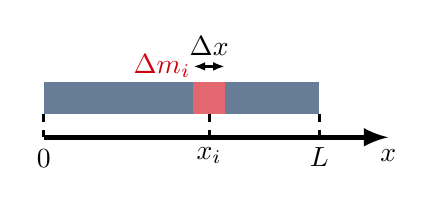
\begin{tikzpicture}[scale=1]
\tikzmath{
\L=3.5;
\w=0.4;
\h=0.3;
\dx=0.2;
}
\scalebox{1.0}{

\fill[myblue!60] (0,\h) rectangle (\L,\h+\w);

\draw[-latex, line width=2] (0,0) node[below] {$0$} -- (1.25*\L,0) node[below] {$x$};
\draw[dashed, line width=1] (0,\h) -- (0,0);
\draw[dashed, line width=1] (\L,\h) -- (\L,0) node[below] {$L$};

\draw[dashed, line width=1] (0.6*\L,\h) -- (0.6*\L,0) node[below] {$x_i$};

\fill[myred!60] (0.6*\L-\dx,\h) rectangle (0.6*\L+\dx,\h+\w);
\draw[{Latex[length=1.5mm]}-{Latex[length=1.5mm]},line width = 1] (0.6*\L-\dx,\h+\w+0.2) -- (0.6*\L+\dx,\h+\w+0.2)node[midway,above]{$\Delta x$};
\node[color=myred] at (0.6*\L-3*\dx,\h+\w+0.2){$\Delta m_i$};
}
\end{tikzpicture}
\captionof*{figure}{\textit{A rod of mass, $M$, and length, $L$, modeled as the sum of many ``mini rods'' of length $\Delta x$ and mass $\Delta m_i$.}}
}

%%%%%%%%%%%%%%%%%%%%%%%%%%%%%%%%
\twocolframest{Example: The mass of a \emph{non-uniform} rod}
{
\begin{itemize}
\scriptsize
\item Suppose the linear density \emph{varies} with position:
\begin{align*}
\mu = \mu(x)
\end{align*}
\item To get the mass of a length, $L$, of rod, we have to sum the masses of $N$ \emph{different} mini-rods:
\begin{align*}
\Delta m_i&=\mu(x_i) \Delta x\\
\therefore M &=\sum_{i=0}^{i=N-1}\Delta m_i =\lim_{\Delta x\to 0} \sum_{i=0}^{i=N-1} \mu(x_i) \Delta x
\end{align*}


\item How do we evaluate this sum? As $\Delta x\to 0$ , there are an infinite number of mini-rods (an infinite number of terms in the sum).
\item Keep in mind that this is the problem that we'd like to solve, as we go and get lost in math.
\end{itemize}
}
{
\centering
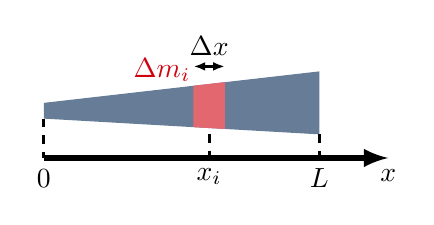
\begin{tikzpicture}[scale=1]
\tikzmath{
\L=3.5;
\w=0.4;
\h=0.3;
\dx=0.2;
\slobot=-\w/2/\L;
\ofsbot=\h+\w/2;
\slotop=\w/\L;
\ofstop=\h+\w;
\xmin=0.6*\L-\dx;
\yminbot=\slobot*\xmin+\ofsbot;
\ymintop=\slotop*\xmin+\ofstop;
\xmax=0.6*\L+\dx;
\ymaxbot=\slobot*\xmax+\ofsbot;
\ymaxtop=\slotop*\xmax+\ofstop;
}
\scalebox{1.0}{

\fill[myblue!60] (0,\h+\w/2) -- (\L,\h) -- (\L,\h+2*\w) -- (0,\h+\w);;

\draw[-latex, line width=2] (0,0) node[below] {$0$} -- (1.25*\L,0) node[below] {$x$};

\draw[dashed, line width=1] (0,\h+\w/2) -- (0,0);
\draw[dashed, line width=1] (\L,\h) -- (\L,0) node[below] {$L$};
\draw[dashed, line width=1] (0.6*\L,\h) -- (0.6*\L,0) node[below] {$x_i$};

\fill[myred!60] (\xmin,\yminbot) -- (\xmax,\ymaxbot) -- (\xmax,\ymaxtop) -- (\xmin,\ymintop);

\draw[{Latex[length=1.5mm]}-{Latex[length=1.5mm]},line width = 1] (\xmin,\ymaxtop+0.2) -- (\xmax,\ymaxtop+0.2)node[midway,above]{$\Delta x$};
\node[color=myred] at (0.6*\L-3*\dx,\ymintop+0.2){$\Delta m_i$};
}
\end{tikzpicture}
\captionof*{figure}{\textit{A non-uniform rod of mass, $M$, and length, $L$, modeled as the sum of many ``mini rods'' of length $\Delta x$ and mass $\Delta m_i$.}}
}


%%%%%%%%%%%%%%%%%%%%%%%%%%%%%%%%
\subsection{The anti-derivative}
\label{subsec:antider}
\begin{bulletframe}{The anti-derivative}
\item Tuesday, we saw that we can determine the rate of change of a function with respect to one (or more) of its independent variables (the derivative).
\item Today, we will see that given the derivative of a function, we can find the original function (the anti-derivative of the function that we are given).
\item Derivative of $f(x)$ with respect to $x$:  
\begin{align*}
f'(x) = \frac{d}{dx} f(x) \quad \text{Take the derivative with respect to x.}
\end{align*}
\item Anti-derivative of $f(x)$ with respect to $x$: 
\begin{align*}
F(x) &= \int f(x) dx \quad \text{Take the anti-derivative with respect to x.}\\
\therefore f(x) &= \frac{d}{dx} F(x)
\end{align*}

\end{bulletframe}


%%%%%%%%%%%%%%%%%%%%%%%%%%%%%%%%




%%%%%%%%%%%%%%%%%%%%%%%%%%%%%%%%
\twocolframest{The constant, $C$}
{

\begin{itemize}
\item Anti-derivatives are only determined up to a constant, $C$.
\item A synonym of anti-derivative is ``indefinite integral'' (since the function is not quite defined unless we specify $C$).
\item In physics, we need functions that describe physical quantities (say, your position along the x-axis as a function of time); those functions need to be fully defined (not up to some constant $C$).
\item The choice of the constant $C$ effectively chooses a point through which the function must pass.
\item It makes sense that the anti-derivative is not fully determined, since all of the functions on the right have the same derivative.
\end{itemize}

}
{
\centering
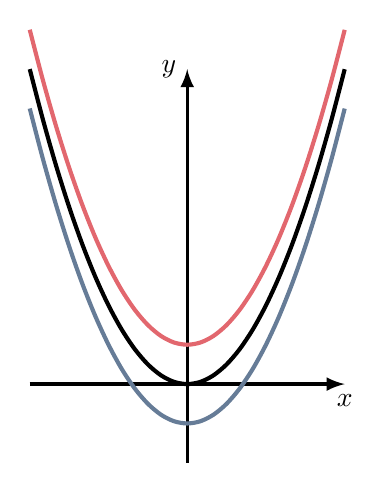
\begin{tikzpicture}[scale=1]
\tikzmath{
}
\scalebox{1.0}{
 
 \draw[-latex, line width=1.25pt] (-2,0) -- (2,0) node[below]{$x$}; 
 \draw[-latex, line width=1.25pt] (0,-1) -- (0,4) node[left]{$y$}; 
 
 %function
 \draw[scale=1, domain=-2.:2., smooth, variable=\x, line width=1.5,color=myblue!60] plot ({\x}, {\x*\x-0.5});
 \draw[scale=1, domain=-2.:2., smooth, variable=\x, line width=1.5] plot ({\x}, {\x*\x});
 \draw[scale=1, domain=-2.:2., smooth, variable=\x, line width=1.5,color=myred!60] plot ({\x}, {\x*\x+0.5});
}
\end{tikzpicture}
\captionof*{figure}{\textit{These functions, $f(x)=x^2+C$ all have the same derivative but different values of $C=\{-0.5,0,0.5\}$. }}
}


%%%%%%%%%%%%%%%%%%%%%%%%%%%%%%%%
\begin{bulletframe} {Determining the anti-derivative of a function} 
\item We would like to determine a function, $F(x)$, knowing:
\begin{itemize}
\item its derivative, $f(x)$.
\item the function must go through a specific point, say $(x_0,F_0)$.
\end{itemize}
\item Physics analogy: we would like to know the position of an object as a function of time, $x(t)$, knowing
\begin{itemize}
\item the velocity of the object as a function of time, $v(t)$ (the time derivative of the position):
\begin{align*}
v(t)=\frac{d}{dt} x(t)
\end{align*}
\item at time $t=t_0$, the object was located at a specific position:
\begin{align*}
x(t_0)=x_0
\end{align*}
\end{itemize}
\end{bulletframe}


%%%%%%%%%%%%%%%%%%%%%%%%%%%%%%%%
\twocolframesf{Graphically, how to visualize an anti-derivative}
{
\begin{itemize}
\item We know:
\begin{itemize}
\item the function $F(x)$ must go through a specific point, $(x_0,F_0)$ .
\item the derivative (slope) of the function at that point, $f(x_0)$.
\end{itemize}
\item<2-> We can determine the next point, $(x_1,F_1)$, through which the function should pass:
\begin{align*}
\frac{\Delta F}{\Delta x} &\approx f(x_0)\quad \text{becomes equal in the}\lim_{\Delta x \to 0}\\
\therefore \Delta F &\approx f(x_0)\Delta x\\
\therefore F_1 &\approx F_0+\Delta F =  F(x_0)+f(x_0)\Delta x
\end{align*}
\item<2->[$\rightarrow$] We now have a method to iterate and find all the points of $F(x)$.
\end{itemize}

}
{
\centering
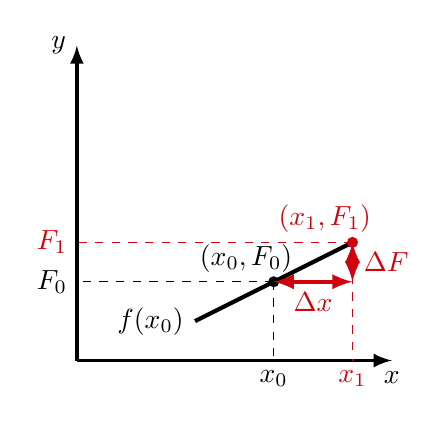
\begin{tikzpicture}[scale=1]
\tikzmath{
\xp=2.5;
\yp=1;
\dx=2;
}
\scalebox{1.0}{

 \coordinate (P) at (\xp,\yp);
 \coordinate (P1) at ($(P)+(\dx/2,0.5*\dx/2)$);
 
 
 \draw[-latex, line width=1.25pt] (0,0) -- (4,0) node[below]{$x$}; 
 \draw[-latex, line width=1.25pt] (0,0) -- (0,4) node[left]{$y$}; 
 
 \fill (P) circle(2pt);
 \node[left=10pt,above] at (P) { $(x_0,F_0)$};
 \draw[dashed] (P) -- +(0,-\yp) node[below]{$x_0$};
 \draw[dashed] (P) -- +(-\xp,0) node[left]{$F_0$};
 
 \draw[line width =1.5] ($(P)-(\dx/2,0.5*\dx/2)$) node[left] {$f(x_0)$} -- ($(P)+(\dx/2,0.5*\dx/2)$) ;
 \only<2->{
  \fill[color=myred] (P1) circle(2pt);
   \node[left=10pt,above,color=myred] at (P1) { $(x_1,F_1)$};
   \draw[dashed,color=myred] (P1) -- +(0,-\yp-0.5*\dx/2) node[below]{$x_1$};
   \draw[dashed,color=myred] (P1) -- +(-\xp-\dx/2,0) node[left]{$F_1$};
   \draw[latex-latex,line width =1.5, color=myred] (P1) -- +(0,-\dx/4) node[midway,right]{$\Delta F$};
   \draw[latex-latex,line width =1.5, color=myred] (P) -- +(\dx/2,0) node[midway,below]{$\Delta x$};
 }
 
}
\end{tikzpicture}
\captionof*{figure}{\textit{The ``shooting method'' for the anti-derivative.}}
}

%%%%%%%%%%%%%%%%%%%%%%%%%%%%%%%%



%%%%%%%%%%%%%%%%%%%%%%%%%%%%%%%%
\begin{bulletframe}{Extending the sum}
\item We have a procedure that allows us to determine the value of the function, $F(x)$, at any value of $x$ (say $x_N$ ):
\begin{align*}
F(x_N) = F(x_0)+f(x_0)\Delta x + f(x_1)\Delta x+ f(x_2)\Delta x+\dots + f(x_{N-1})\Delta x
\end{align*}
where $x_N=x_0+N\Delta x$
\item Using the summation notation and taking the limit:
\begin{align*}
F(x_N) = F(x_0)+\lim_{\Delta x \to 0}\sum_{i=0}^{N-1}f(x_i)\Delta x
\end{align*}
\end{bulletframe}


%%%%%%%%%%%%%%%%%%%%%%%%%%%%%%%%
\subsection{The indefinite and definite integrals}
\label{subsec:indefanddefintegrals}
\begin{bulletframe}{The indefinite and definite integrals}
\item We can re-write the sum as the difference in the anti-derivative evaluated at $x_N$ and $x_0$:
\begin{align*}
F(x_N) - F(x_0)=\lim_{\Delta x \to 0}\sum_{i=0}^{N-1}f(x_i)\Delta x
\end{align*}
The constant, $C$, in the anti-derivative cancels when we take this difference.
\item We call this difference the ``\textbf{definite integral (or just integral) of $f(x)$ from $x_0$  to $x_N$}'', and use the following notation:
\begin{align*}
\Aboxed{F(x_N) - F(x_0)=\int_{x_0}^{x_N}f(x)dx}
\end{align*}
\item Note the ``limits'' on the integral, which differentiates this from the anti-derivative.
\end{bulletframe}


%%%%%%%%%%%%%%%%%%%%%%%%%%%%%%%%
\begin{bulletframe}{Definite vs indefinite}
\item Given the function, $f(x)=x^2$
\item The indefinite integral (or anti-derivative) is a \textbf{function}:
\begin{align*}
F(x) = \int f(x) dx=\int x^2dx = \frac{1}{3}x^3+C
\end{align*}
\item The definite integral between $x=1$ and $x=3$ is a \textbf{number}:
\begin{align*}
\int_1^3x^2dx = F(3) - F(1) = \frac{1}{3}3^3-\frac{1}{3}1^3=9-\frac{1}{3}=\frac{26}{3}
\end{align*}
Note that the $C$ cancels in the subtraction.
\item Physical quantities in physics must be given by definite integrals.
\end{bulletframe}


%%%%%%%%%%%%%%%%%%%%%%%%%%%%%%%%
\subsection{How to determine the anti-derivative}
\label{subsec:determiningantider}
\twocolframe{How to determine the anti-derivative}
{
\begin{itemize}
\item To determine the anti-derivative of a function, $f(x)$, we need to be able to evaluate the sum:
\begin{align*}
\lim_{\Delta x \to 0}\sum_{i=0}^{N-1}f(x_i)\Delta x
\end{align*}
\item The textbook shows you how to do it for $f(x)=2x$. Your calculus course will show you how to do it for other functions...
\end{itemize}
}
{
\begin{center}
\scriptsize
\begin{tabular}{l l}
\textbf{Function, $f(x)$} & \textbf{Anti-derivative, $F(x)$}\\
\hline\hline
$f(x)=a$ & $F(x)=ax+C$ \\
$f(x)=x^n$ & $F(x)=\frac{1}{n+1}x^{n+1}+C$ \\
$f(x)=\frac{1}{x}$ & $F(x)=\ln(|x|)+C$ \\
$f(x)=\sin(x)$ & $F(x)=-\cos(x)+C$ \\
$f(x)=\cos(x)$ & $F(x)=\sin(x)+C$ \\
$f(x)=\tan(x)$ & $F(x)=-\ln(|\cos(x)|)+C$ \\
$f(x)=e^x$ & $F(x)=e^x+C$ \\
$f(x)=\ln(x)$ & $F(x)=x\ln(x)-x+C$ \\
\hline
\end{tabular}
\captionof*{table}{\label{tab:Calculus:commonints}Common indefinite integrals of functions. Unlike derivatives, for which you can always determine an analytical function, you cannot always determine an analytical form for the indefinite integral of a function. }
\end{center}
}



%%%%%%%%%%%%%%%%%%%%%%%%%%%%%%%%
%%%%%%%%%%%%%%%%%%%%%%%%%%%%%%%%
\twocolframesf{Graphical representation of the sum}
{
\scriptsize
\begin{itemize}
\item If we graph $f(x)$ we can see that each term in the sum for the integral corresponds to the area of a little rectangle under the function $f(x)$:
\begin{align*}
\lim_{\Delta x \to 0}\sum_{i=0}^{N-1}f(x_i)\Delta x = f(x_0)\Delta x + f(x_1)\Delta x\\
+ f(x_2)\Delta x+\dots + f(x_{N-1})\Delta x
\end{align*}
\item The definite integral:
\begin{align*}
\int_{x_0}^{X_N}f(x) dx=\lim_{\Delta x \to 0}\sum_{i=0}^{N-1}f(x_i)\Delta x 
\end{align*}
is thus the total area underneath $f(x)$, between $x_0$ and $x_N$  
\end{itemize}

}
{
\centering
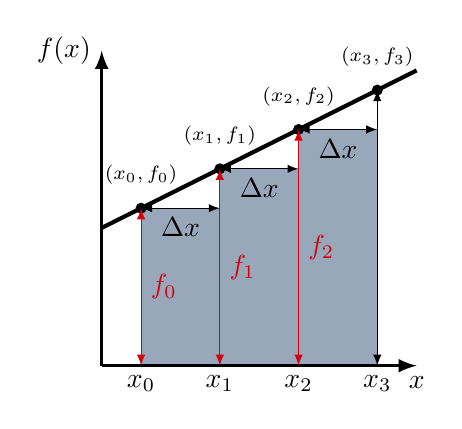
\begin{tikzpicture}[scale=1]
\tikzmath{
\xp=0.5;
\yp=2;
\dx=2;
}
\scalebox{1.0}{

 \coordinate (P) at (\xp,\yp);
 \coordinate (P1) at ($(P)+(\dx/2,0.5*\dx/2)$);
 \coordinate (P2) at ($(P)+2*(\dx/2,0.5*\dx/2)$);
 \coordinate (P3) at ($(P)+3*(\dx/2,0.5*\dx/2)$);
 
 \fill[color=myblue!40] (P) rectangle ($(P1)+(0,-\yp-0.5*\dx/2)$);
 \fill[color=myblue!40] (P1) rectangle ($(P2)+(0,-\yp-0.5*\dx)$);
 \fill[color=myblue!40] (P2) rectangle ($(P3)+(0,-\yp-0.75*\dx)$);
  
 
 \draw[-latex, line width=1.25pt] (0,0) -- (4,0) node[below]{$x$}; 
 \draw[-latex, line width=1.25pt] (0,0) -- (0,4) node[left]{$f(x)$}; 
 

 \draw[line width =1.5] ($(P)-0.5*(\dx/2,0.5*\dx/2)$)-- ($(P)+3.5*(\dx/2,0.5*\dx/2)$) ;
 
 \fill (P) circle(2pt);
 \draw[latex-latex,color=myred] (P) -- +(0,-\yp) node[below,color=black]{$x_0$} node[midway,right] {$f_0$};

 \fill (P1) circle(2pt);
 \draw[latex-latex,color=myred] (P1) -- +(0,-\yp-0.5*\dx/2) node[below,color=black]{$x_1$} node[midway,right] {$f_1$};

 \fill (P2) circle(2pt);
 \draw[latex-latex,color=myred] (P2) -- +(0,-\yp-0.5*\dx) node[below,color=black]{$x_2$} node[midway,right] {$f_2$};

 \fill (P3) circle(2pt);
 \draw[latex-latex] (P3) -- +(0,-\yp-0.75*\dx) node[below]{$x_3$} ;
 
 
 \draw[latex-latex] (P) -- +(\dx/2,0) node[midway,below] {$\Delta x$};
 \draw[latex-latex] (P1) -- +(\dx/2,0) node[midway,below] {$\Delta x$};
 \draw[latex-latex] (P2) -- +(\dx/2,0) node[midway,below] {$\Delta x$};

 \node[above=5pt] at (P) {\scriptsize $(x_0,f_0)$}; 
 \node[above=5pt] at (P1) {\scriptsize $(x_1,f_1)$};
 \node[above=5pt] at (P2) {\scriptsize $(x_2,f_2)$};
 \node[above=5pt] at (P3) {\scriptsize $(x_3,f_3)$};
 
}
\end{tikzpicture}
\captionof*{figure}{\textit{Each rectangle has an area $f(x_i) \Delta x$. As $\Delta x\to 0$, the rectangles correspond to the area under $f(x)$.}}
}



%%%%%%%%%%%%%%%%%%%%%%%%%%%%%%%%
%%%%%%%%%%%%%%%%%%%%%%%%%%%%%%%%
\subsection{Back to physiscs: the mass of a non-uniform rod}
\label{subsec:btpnonunirodmass}
\twocolframest{Back to physics: The mass of a \emph{non-uniform} rod}
{
\begin{itemize}
\scriptsize
\item Suppose the linear density \emph{varies} with position:
\begin{align*}
\mu = \mu(x)
\end{align*}
\item To get the mass of a length $L$ of rod, we have to sum the masses of $N$ \emph{different} mini-rods:
\begin{align*}
M &=\sum_{i=0}^{i=N-1}\Delta m_i =\lim_{\Delta x\to 0} \sum_{i=0}^{i=N-1} \mu(x_i) \Delta x
\end{align*}
\item The sum, is given by the definite integral:
\begin{align*}
\lim_{\Delta x\to 0} \sum_{i=0}^{i=N-1} \mu(x_i) \Delta x=\int_{x=0}^{x=L}\mu(x)dx
\end{align*}
If we know $\mu(x)$, we can ask our math friends for the anti-derivative of that function.
\end{itemize}

}
{
\begin{center}
\vspace{-1cm}
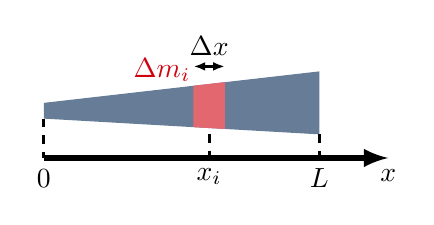
\begin{tikzpicture}[scale=1]
\tikzmath{
\L=3.5;
\w=0.4;
\h=0.3;
\dx=0.2;
\slobot=-\w/2/\L;
\ofsbot=\h+\w/2;
\slotop=\w/\L;
\ofstop=\h+\w;
\xmin=0.6*\L-\dx;
\yminbot=\slobot*\xmin+\ofsbot;
\ymintop=\slotop*\xmin+\ofstop;
\xmax=0.6*\L+\dx;
\ymaxbot=\slobot*\xmax+\ofsbot;
\ymaxtop=\slotop*\xmax+\ofstop;
}
\scalebox{1.0}{

\fill[myblue!60] (0,\h+\w/2) -- (\L,\h) -- (\L,\h+2*\w) -- (0,\h+\w);;

\draw[-latex, line width=2] (0,0) node[below] {$0$} -- (1.25*\L,0) node[below] {$x$};

\draw[dashed, line width=1] (0,\h+\w/2) -- (0,0);
\draw[dashed, line width=1] (\L,\h) -- (\L,0) node[below] {$L$};
\draw[dashed, line width=1] (0.6*\L,\h) -- (0.6*\L,0) node[below] {$x_i$};

\fill[myred!60] (\xmin,\yminbot) -- (\xmax,\ymaxbot) -- (\xmax,\ymaxtop) -- (\xmin,\ymintop);

\draw[{Latex[length=1.5mm]}-{Latex[length=1.5mm]},line width = 1] (\xmin,\ymaxtop+0.2) -- (\xmax,\ymaxtop+0.2)node[midway,above]{$\Delta x$};
\node[color=myred] at (0.6*\L-3*\dx,\ymintop+0.2){$\Delta m_i$};
}
\end{tikzpicture}
\captionof*{figure}{\textit{A non-uniform rod of mass, $M$, and length, $L$, modeled as the sum of many ``mini rods'' of length $\Delta x$ and mass $\Delta m_i$.}}
\end{center}
\only<2>{
\scriptsize
\color{myblue!60}{As physicists, we need a tool to be able to calculate these sums.\\
The mathematicians (well actually...) have developed this tool from calculus that can find the anti-derivative of a function.\\
It turns out that this tool also gives a way to calculate the sums that we need in physics!}
}
}


%%%%%%%%%%%%%%%%%%%%%%%%%%%%%%%%
\begin{frame}{Back to physics: The mass of a \emph{non-uniform} rod}
\begin{itemize}
\item Suppose that $\mu(x)=2ax$, then we (our math friends) know that:
\begin{align*}
F(x) = \int \mu(x) dx = ax^2+C
\end{align*}
\item We want:
\begin{align*}
\lim_{\Delta x\to 0} \sum_{i=0}^{i=N} \mu(x_i) \Delta x=\int_{x=0}^{x=L}\mu(x)dx
\end{align*}
\item We can thus evaluate:
\begin{align*}
\int_{x=0}^{x=L}\mu(x)dx = F(x=L)-F(x=0) = aL^2 - 0 = aL^2
\end{align*}
\end{itemize}
\end{frame}


%%%%%%%%%%%%%%%%%%%%%%%%%%%%%%%%
\twocolframest{The infinitesimals}
{
\begin{itemize}
\scriptsize
\item We can think of an \textit{infinitesimally small} rod of mass, $dm$, and length, $dx$:
\begin{align*}
dm = \mu(x) dx
\end{align*}
\item The total mass of the rod, $M$, is the sum of the masses of the infinitesimal rods:
\begin{align*}
M = \sum dm = \int_0^M dm= \int_0^L\mu(x) dx
\end{align*}
\item With practice, you will get used to just writing everything with infinitesimals rather than a sum and taking the limits!
\item This also makes it clear that \textbf{an integral is a sum}
\end{itemize}

}
{
\vspace{-1cm}
\begin{center}

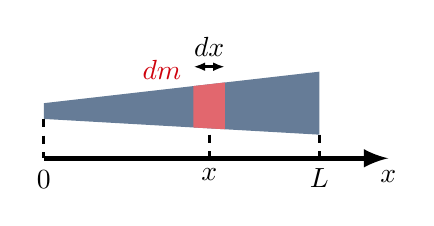
\begin{tikzpicture}[scale=1]
\tikzmath{
\L=3.5;
\w=0.4;
\h=0.3;
\dx=0.2;
\slobot=-\w/2/\L;
\ofsbot=\h+\w/2;
\slotop=\w/\L;
\ofstop=\h+\w;
\xmin=0.6*\L-\dx;
\yminbot=\slobot*\xmin+\ofsbot;
\ymintop=\slotop*\xmin+\ofstop;
\xmax=0.6*\L+\dx;
\ymaxbot=\slobot*\xmax+\ofsbot;
\ymaxtop=\slotop*\xmax+\ofstop;
}
\scalebox{1.0}{

\fill[myblue!60] (0,\h+\w/2) -- (\L,\h) -- (\L,\h+2*\w) -- (0,\h+\w);;

\draw[-latex, line width=2] (0,0) node[below] {$0$} -- (1.25*\L,0) node[below] {$x$};

\draw[dashed, line width=1] (0,\h+\w/2) -- (0,0);
\draw[dashed, line width=1] (\L,\h) -- (\L,0) node[below] {$L$};
\draw[dashed, line width=1] (0.6*\L,\h) -- (0.6*\L,0) node[below] {$x$};

\fill[myred!60] (\xmin,\yminbot) -- (\xmax,\ymaxbot) -- (\xmax,\ymaxtop) -- (\xmin,\ymintop);

\draw[{Latex[length=1.5mm]}-{Latex[length=1.5mm]},line width = 1] (\xmin,\ymaxtop+0.2) -- (\xmax,\ymaxtop+0.2)node[midway,above]{$dx$};
\node[color=myred] at (0.6*\L-3*\dx,\ymintop+0.2){$dm$};
}
\end{tikzpicture}
\captionof*{figure}{\textit{A non-uniform rod of mass, $M$, and length, $L$, modeled as the sum of many ``mini rods'' of length $\Delta x$ and mass $\Delta m_i$.}}
\end{center}
\scriptsize
Compare with:
\begin{align*}
\Delta m_i &= \mu(x) \Delta x\\
M &=\sum_{i=0}^{i=N}\Delta m_i 
=\lim_{\Delta x\to 0} \sum_{i=0}^{i=N-1} \mu(x_i) \Delta x
\end{align*}
}


%%%%%%%%%%%%%%%%%%%%%%%%%%%%%%%%



%%%%%%%%%%%%%%%%%%%%%%%%%%%%%%%%



%%%%%%%%%%%%%%%%%%%%%%%%%%%%%%%%



%%%%%%%%%%%%%%%%%%%%%%%%%%%%%%%%



%%%%%%%%%%%%%%%%%%%%%%%%%%%%%%%%



%%%%%%%%%%%%%%%%%%%%%%%%%%%%%%%%



%%%%%%%%%%%%%%%%%%%%%%%%%%%%%%%%



%%%%%%%%%%%%%%%%%%%%%%%%%%%%%%%%



%%%%%%%%%%%%%%%%%%%%%%%%%%%%%%%%






\end{document}


